\documentclass[a4paper]{article}
\usepackage[]{graphicx}\usepackage[]{xcolor}
% maxwidth is the original width if it is less than linewidth
% otherwise use linewidth (to make sure the graphics do not exceed the margin)
\makeatletter
\def\maxwidth{ %
  \ifdim\Gin@nat@width>\linewidth
    \linewidth
  \else
    \Gin@nat@width
  \fi
}
\makeatother

\definecolor{fgcolor}{rgb}{0.345, 0.345, 0.345}
\newcommand{\hlnum}[1]{\textcolor[rgb]{0.686,0.059,0.569}{#1}}%
\newcommand{\hlstr}[1]{\textcolor[rgb]{0.192,0.494,0.8}{#1}}%
\newcommand{\hlcom}[1]{\textcolor[rgb]{0.678,0.584,0.686}{\textit{#1}}}%
\newcommand{\hlopt}[1]{\textcolor[rgb]{0,0,0}{#1}}%
\newcommand{\hlstd}[1]{\textcolor[rgb]{0.345,0.345,0.345}{#1}}%
\newcommand{\hlkwa}[1]{\textcolor[rgb]{0.161,0.373,0.58}{\textbf{#1}}}%
\newcommand{\hlkwb}[1]{\textcolor[rgb]{0.69,0.353,0.396}{#1}}%
\newcommand{\hlkwc}[1]{\textcolor[rgb]{0.333,0.667,0.333}{#1}}%
\newcommand{\hlkwd}[1]{\textcolor[rgb]{0.737,0.353,0.396}{\textbf{#1}}}%
\let\hlipl\hlkwb

\usepackage{framed}
\makeatletter
\newenvironment{kframe}{%
 \def\at@end@of@kframe{}%
 \ifinner\ifhmode%
  \def\at@end@of@kframe{\end{minipage}}%
  \begin{minipage}{\columnwidth}%
 \fi\fi%
 \def\FrameCommand##1{\hskip\@totalleftmargin \hskip-\fboxsep
 \colorbox{shadecolor}{##1}\hskip-\fboxsep
     % There is no \\@totalrightmargin, so:
     \hskip-\linewidth \hskip-\@totalleftmargin \hskip\columnwidth}%
 \MakeFramed {\advance\hsize-\width
   \@totalleftmargin\z@ \linewidth\hsize
   \@setminipage}}%
 {\par\unskip\endMakeFramed%
 \at@end@of@kframe}
\makeatother

\definecolor{shadecolor}{rgb}{.97, .97, .97}
\definecolor{messagecolor}{rgb}{0, 0, 0}
\definecolor{warningcolor}{rgb}{1, 0, 1}
\definecolor{errorcolor}{rgb}{1, 0, 0}
\newenvironment{knitrout}{}{} % an empty environment to be redefined in TeX

\usepackage{alltt}
\newcommand{\SweaveOpts}[1]{}  % do not interfere with LaTeX
\newcommand{\SweaveInput}[1]{} % because they are not real TeX commands
\newcommand{\Sexpr}[1]{}       % will only be parsed by R




\usepackage[utf8]{inputenc}
%\usepackage[ngerman]{babel}
\usepackage{a4wide,paralist}
\usepackage{amsmath, amssymb, xfrac, amsthm}
\usepackage{dsfont}
%\usepackage[usenames,dvipsnames]{xcolor}
\usepackage{xcolor}
\usepackage{amsfonts}
\usepackage{graphicx}
\usepackage{caption}
\usepackage{subcaption}
\usepackage{framed}
\usepackage{multirow}
\usepackage{bytefield}
\usepackage{csquotes}
\usepackage[breakable, theorems, skins]{tcolorbox}
\usepackage{hyperref}
\usepackage{cancel}
\usepackage{bm}
\usepackage{algorithm}
\usepackage{algpseudocode}


% Rarely used fontstyle for R packages, used only in 
% - forests/slides-forests-benchmark.tex
% - exercises/single-exercises/methods_l_1.Rnw
% - slides/cart/attic/slides_extra_trees.Rnw
\newcommand{\pkg}[1]{{\fontseries{b}\selectfont #1}}

% Spacing helpers, used often (mostly in exercises for \dlz)
\newcommand{\lz}{\vspace{0.5cm}} % vertical space (used often in slides)
\newcommand{\dlz}{\vspace{1cm}}  % double vertical space (used often in exercises, never in slides)

%--------------------%
%  New environments  %
%--------------------%

 % Frame with breaks and verbatim // this is used very often
\newenvironment{vbframe}
{
\begin{frame}[containsverbatim,allowframebreaks]
}
{
\end{frame}
}

% Frame with verbatim without breaks (to avoid numbering one slided frames)
% This is not used anywhere but I can see it being useful
\newenvironment{vframe}
{
\begin{frame}[containsverbatim]
}
{
\end{frame}
}

% Itemize block
\newenvironment{blocki}[1]
{
\begin{block}{#1}\begin{itemize}
}
{
\end{itemize}\end{block}
}

% textcolor that works in mathmode
% https://tex.stackexchange.com/a/261480
% Used e.g. in forests/slides-forests-bagging.tex
% [...] \textcolor{blue}{\tfrac{1}{M}\sum^M_{m} [...]
% \makeatletter
% \renewcommand*{\@textcolor}[3]{%
%   \protect\leavevmode
%   \begingroup
%     \color#1{#2}#3%
%   \endgroup
% }
% \makeatother


\tcbset{enhanced}

\DeclareRobustCommand{\mybox}[2][gray!20]{%
	\iffalse
	\begin{tcolorbox}[   %% Adjust the following parameters at will.
		breakable,
		left=0pt,
		right=0pt,
		top=0pt,
		bottom=0pt,
		colback=#1,
		colframe=#1,
		width=\dimexpr\linewidth\relax,
		enlarge left by=0mm,
		boxsep=5pt,
		arc=0pt,outer arc=0pt,
		]
		#2
	\end{tcolorbox}
	\fi
}

\DeclareRobustCommand{\myboxshow}[2][gray!20]{%
%	\iffalse
	\begin{tcolorbox}[   %% Adjust the following parameters at will.
		breakable,
		left=0pt,
		right=0pt,
		top=0pt,
		bottom=0pt,
		colback=#1,
		colframe=#1,
		width=\dimexpr\linewidth\relax,
		enlarge left by=0mm,
		boxsep=5pt,
		arc=0pt,outer arc=0pt,
		]
		#2
	\end{tcolorbox}
%	\fi
}


%exercise numbering
\renewcommand{\theenumi}{(\alph{enumi})}
\renewcommand{\theenumii}{\roman{enumii}}
\renewcommand\labelenumi{\theenumi}


\font \sfbold=cmssbx10

\setlength{\oddsidemargin}{0cm} \setlength{\textwidth}{16cm}


\sloppy
\parindent0em
\parskip0.5em
\topmargin-2.3 cm
\textheight25cm
\textwidth17.5cm
\oddsidemargin-0.8cm
\pagestyle{empty}

\newcommand{\kopf}[2]{
\hrule
\vspace{.15cm}
\begin{minipage}{\textwidth}
%akwardly i had to put \" here to make it compile correctly
	{\sf\bf Introduction to Machine Learning \hfill Exercise sheet #1\\
	 \url{https://slds-lmu.github.io/i2ml/} \hfill #2}
\end{minipage}
\vspace{.05cm}
\hrule
\vspace{1cm}}

\newcommand{\kopfic}[2]{
\hrule
\vspace{.15cm}
\begin{minipage}{\textwidth}
%akwardly i had to put \" here to make it compile correctly
	{\sf\bf Introduction to Machine Learning \hfill Live Session #1\\
	 \url{https://slds-lmu.github.io/i2ml/} \hfill #2}
\end{minipage}
\vspace{.05cm}
\hrule
\vspace{1cm}}

\newcommand{\kopficsl}[2]{
\hrule
\vspace{.15cm}
\begin{minipage}{\textwidth}
%akwardly i had to put \" here to make it compile correctly
	{\sf\bf Supervised Learning \hfill Live Session #1\\
	 \url{https://slds-lmu.github.io/i2ml/} \hfill #2}
\end{minipage}
\vspace{.05cm}
\hrule
\vspace{1cm}}

\newcommand{\kopfaml}[2]{
\hrule
\vspace{.15cm}
\begin{minipage}{\textwidth}
%akwardly i had to put \" here to make it compile correctly
	{\sf\bf Advanced Machine Learning \hfill Exercise sheet #1\\
	 \url{https://slds-lmu.github.io/i2ml/} \hfill #2}
\end{minipage}
\vspace{.05cm}
\hrule
\vspace{1cm}}


\newcommand{\kopfdive}[1]{
\hrule
\vspace{.15cm}
\begin{minipage}{\textwidth}
%akwardly i had to put \" here to make it compile correctly
	{\sf\bf Supervised Learning \hfill Deep Dive\\
	 \url{https://slds-lmu.github.io/i2ml/} \hfill #1}
\end{minipage}
\vspace{.05cm}
\hrule
\vspace{1cm}}

\newcommand{\kopfsl}[2]{
\hrule
\vspace{.15cm}
\begin{minipage}{\textwidth}
%akwardly i had to put \" here to make it compile correctly
	{\sf\bf Supervised Learning \hfill Exercise sheet #1\\
	 \url{https://slds-lmu.github.io/i2ml/} \hfill #2}
\end{minipage}
\vspace{.05cm}
\hrule
\vspace{1cm}}

\newenvironment{allgemein}
	{\noindent}{\vspace{1cm}}

\newcounter{aufg}
\newenvironment{aufgabe}[1]
	{\refstepcounter{aufg}\textbf{Exercise \arabic{aufg}: #1}\\ \noindent}
	{\vspace{0.5cm}}

\newcounter{loes}
\newenvironment{loesung}[1]
	{\refstepcounter{loes}\textbf{Solution \arabic{loes}: #1}\\\noindent}
	{\bigskip}

\newenvironment{bonusaufgabe}
	{\refstepcounter{aufg}\textbf{Exercise \arabic{aufg}*\footnote{This
	is a bonus exercise.}:}\\ \noindent}
	{\vspace{0.5cm}}

\newenvironment{bonusloesung}
	{\refstepcounter{loes}\textbf{Solution \arabic{loes}*:}\\\noindent}
	{\bigskip}



\begin{document}
% !Rnw weave = knitr



% dependencies: amsmath, amssymb, dsfont
% math spaces
\ifdefined\N
\renewcommand{\N}{\mathds{N}} % N, naturals
\else \newcommand{\N}{\mathds{N}} \fi
\newcommand{\Z}{\mathds{Z}} % Z, integers
\newcommand{\Q}{\mathds{Q}} % Q, rationals
\newcommand{\R}{\mathds{R}} % R, reals
\ifdefined\C
\renewcommand{\C}{\mathds{C}} % C, complex
\else \newcommand{\C}{\mathds{C}} \fi
\newcommand{\continuous}{\mathcal{C}} % C, space of continuous functions
\newcommand{\M}{\mathcal{M}} % machine numbers
\newcommand{\epsm}{\epsilon_m} % maximum error

% counting / finite sets
\newcommand{\setzo}{\{0, 1\}} % set 0, 1
\newcommand{\setmp}{\{-1, +1\}} % set -1, 1
\newcommand{\unitint}{[0, 1]} % unit interval

% basic math stuff
\newcommand{\xt}{\tilde x} % x tilde
\DeclareMathOperator*{\argmax}{arg\,max} % argmax
\DeclareMathOperator*{\argmin}{arg\,min} % argmin
\newcommand{\argminlim}{\mathop{\mathrm{arg\,min}}\limits} % argmax with limits
\newcommand{\argmaxlim}{\mathop{\mathrm{arg\,max}}\limits} % argmin with limits
\newcommand{\sign}{\operatorname{sign}} % sign, signum
\newcommand{\I}{\mathbb{I}} % I, indicator
\newcommand{\order}{\mathcal{O}} % O, order
\newcommand{\bigO}{\mathcal{O}} % Big-O Landau
\newcommand{\littleo}{{o}} % Little-o Landau
\newcommand{\pd}[2]{\frac{\partial{#1}}{\partial #2}} % partial derivative
\newcommand{\floorlr}[1]{\left\lfloor #1 \right\rfloor} % floor
\newcommand{\ceillr}[1]{\left\lceil #1 \right\rceil} % ceiling
\newcommand{\indep}{\perp \!\!\! \perp} % independence symbol

% sums and products
\newcommand{\sumin}{\sum\limits_{i=1}^n} % summation from i=1 to n
\newcommand{\sumim}{\sum\limits_{i=1}^m} % summation from i=1 to m
\newcommand{\sumjn}{\sum\limits_{j=1}^n} % summation from j=1 to p
\newcommand{\sumjp}{\sum\limits_{j=1}^p} % summation from j=1 to p
\newcommand{\sumik}{\sum\limits_{i=1}^k} % summation from i=1 to k
\newcommand{\sumkg}{\sum\limits_{k=1}^g} % summation from k=1 to g
\newcommand{\sumjg}{\sum\limits_{j=1}^g} % summation from j=1 to g
\newcommand{\meanin}{\frac{1}{n} \sum\limits_{i=1}^n} % mean from i=1 to n
\newcommand{\meanim}{\frac{1}{m} \sum\limits_{i=1}^m} % mean from i=1 to n
\newcommand{\meankg}{\frac{1}{g} \sum\limits_{k=1}^g} % mean from k=1 to g
\newcommand{\prodin}{\prod\limits_{i=1}^n} % product from i=1 to n
\newcommand{\prodkg}{\prod\limits_{k=1}^g} % product from k=1 to g
\newcommand{\prodjp}{\prod\limits_{j=1}^p} % product from j=1 to p

% linear algebra
\newcommand{\one}{\bm{1}} % 1, unitvector
\newcommand{\zero}{\mathbf{0}} % 0-vector
\newcommand{\id}{\bm{I}} % I, identity
\newcommand{\diag}{\operatorname{diag}} % diag, diagonal
\newcommand{\trace}{\operatorname{tr}} % tr, trace
\newcommand{\spn}{\operatorname{span}} % span
\newcommand{\scp}[2]{\left\langle #1, #2 \right\rangle} % <.,.>, scalarproduct
\newcommand{\mat}[1]{\begin{pmatrix} #1 \end{pmatrix}} % short pmatrix command
\newcommand{\Amat}{\mathbf{A}} % matrix A
\newcommand{\Deltab}{\mathbf{\Delta}} % error term for vectors

% basic probability + stats
\renewcommand{\P}{\mathds{P}} % P, probability
\newcommand{\E}{\mathds{E}} % E, expectation
\newcommand{\var}{\mathsf{Var}} % Var, variance
\newcommand{\cov}{\mathsf{Cov}} % Cov, covariance
\newcommand{\corr}{\mathsf{Corr}} % Corr, correlation
\newcommand{\normal}{\mathcal{N}} % N of the normal distribution
\newcommand{\iid}{\overset{i.i.d}{\sim}} % dist with i.i.d superscript
\newcommand{\distas}[1]{\overset{#1}{\sim}} % ... is distributed as ...

% machine learning
\newcommand{\Xspace}{\mathcal{X}} % X, input space
\newcommand{\Yspace}{\mathcal{Y}} % Y, output space
\newcommand{\Zspace}{\mathcal{Z}} % Space of sampled datapoints ! Also defined identically in ml-online.tex !
\newcommand{\nset}{\{1, \ldots, n\}} % set from 1 to n
\newcommand{\pset}{\{1, \ldots, p\}} % set from 1 to p
\newcommand{\gset}{\{1, \ldots, g\}} % set from 1 to g
\newcommand{\Pxy}{\mathbb{P}_{xy}} % P_xy
\newcommand{\Exy}{\mathbb{E}_{xy}} % E_xy: Expectation over random variables xy
\newcommand{\xv}{\mathbf{x}} % vector x (bold)
\newcommand{\xtil}{\tilde{\mathbf{x}}} % vector x-tilde (bold)
\newcommand{\yv}{\mathbf{y}} % vector y (bold)
\newcommand{\xy}{(\xv, y)} % observation (x, y)
\newcommand{\xvec}{\left(x_1, \ldots, x_p\right)^\top} % (x1, ..., xp)
\newcommand{\Xmat}{\mathbf{X}} % Design matrix
\newcommand{\allDatasets}{\mathds{D}} % The set of all datasets
\newcommand{\allDatasetsn}{\mathds{D}_n}  % The set of all datasets of size n
\newcommand{\D}{\mathcal{D}} % D, data
\newcommand{\Dn}{\D_n} % D_n, data of size n
\newcommand{\Dtrain}{\mathcal{D}_{\text{train}}} % D_train, training set
\newcommand{\Dtest}{\mathcal{D}_{\text{test}}} % D_test, test set
\newcommand{\xyi}[1][i]{\left(\xv^{(#1)}, y^{(#1)}\right)} % (x^i, y^i), i-th observation
\newcommand{\Dset}{\left( \xyi[1], \ldots, \xyi[n]\right)} % {(x1,y1)), ..., (xn,yn)}, data
\newcommand{\defAllDatasetsn}{(\Xspace \times \Yspace)^n} % Def. of the set of all datasets of size n
\newcommand{\defAllDatasets}{\bigcup_{n \in \N}(\Xspace \times \Yspace)^n} % Def. of the set of all datasets
\newcommand{\xdat}{\left\{ \xv^{(1)}, \ldots, \xv^{(n)}\right\}} % {x1, ..., xn}, input data
\newcommand{\ydat}{\left\{ \yv^{(1)}, \ldots, \yv^{(n)}\right\}} % {y1, ..., yn}, input data
\newcommand{\yvec}{\left(y^{(1)}, \hdots, y^{(n)}\right)^\top} % (y1, ..., yn), vector of outcomes
\renewcommand{\xi}[1][i]{\xv^{(#1)}} % x^i, i-th observed value of x
\newcommand{\yi}[1][i]{y^{(#1)}} % y^i, i-th observed value of y
\newcommand{\xivec}{\left(x^{(i)}_1, \ldots, x^{(i)}_p\right)^\top} % (x1^i, ..., xp^i), i-th observation vector
\newcommand{\xj}{\xv_j} % x_j, j-th feature
\newcommand{\xjvec}{\left(x^{(1)}_j, \ldots, x^{(n)}_j\right)^\top} % (x^1_j, ..., x^n_j), j-th feature vector
\newcommand{\phiv}{\mathbf{\phi}} % Basis transformation function phi
\newcommand{\phixi}{\mathbf{\phi}^{(i)}} % Basis transformation of xi: phi^i := phi(xi)

%%%%%% ml - models general
\newcommand{\lamv}{\bm{\lambda}} % lambda vector, hyperconfiguration vector
\newcommand{\Lam}{\bm{\Lambda}}	 % Lambda, space of all hpos
% Inducer / Inducing algorithm
\newcommand{\preimageInducer}{\left(\defAllDatasets\right)\times\Lam} % Set of all datasets times the hyperparameter space
\newcommand{\preimageInducerShort}{\allDatasets\times\Lam} % Set of all datasets times the hyperparameter space
% Inducer / Inducing algorithm
\newcommand{\ind}{\mathcal{I}} % Inducer, inducing algorithm, learning algorithm

% continuous prediction function f
\newcommand{\ftrue}{f_{\text{true}}}  % True underlying function (if a statistical model is assumed)
\newcommand{\ftruex}{\ftrue(\xv)} % True underlying function (if a statistical model is assumed)
\newcommand{\fx}{f(\xv)} % f(x), continuous prediction function
\newcommand{\fdomains}{f: \Xspace \rightarrow \R^g} % f with domain and co-domain
\newcommand{\Hspace}{\mathcal{H}} % hypothesis space where f is from
\newcommand{\fbayes}{f^{\ast}} % Bayes-optimal model
\newcommand{\fxbayes}{f^{\ast}(\xv)} % Bayes-optimal model
\newcommand{\fkx}[1][k]{f_{#1}(\xv)} % f_j(x), discriminant component function
\newcommand{\fh}{\hat{f}} % f hat, estimated prediction function
\newcommand{\fxh}{\fh(\xv)} % fhat(x)
\newcommand{\fxt}{f(\xv ~|~ \thetab)} % f(x | theta)
\newcommand{\fxi}{f\left(\xv^{(i)}\right)} % f(x^(i))
\newcommand{\fxih}{\hat{f}\left(\xv^{(i)}\right)} % f(x^(i))
\newcommand{\fxit}{f\left(\xv^{(i)} ~|~ \thetab\right)} % f(x^(i) | theta)
\newcommand{\fhD}{\fh_{\D}} % fhat_D, estimate of f based on D
\newcommand{\fhDtrain}{\fh_{\Dtrain}} % fhat_Dtrain, estimate of f based on D
\newcommand{\fhDnlam}{\fh_{\Dn, \lamv}} %model learned on Dn with hp lambda
\newcommand{\fhDlam}{\fh_{\D, \lamv}} %model learned on D with hp lambda
\newcommand{\fhDnlams}{\fh_{\Dn, \lamv^\ast}} %model learned on Dn with optimal hp lambda
\newcommand{\fhDlams}{\fh_{\D, \lamv^\ast}} %model learned on D with optimal hp lambda

% discrete prediction function h
\newcommand{\hx}{h(\xv)} % h(x), discrete prediction function
\newcommand{\hh}{\hat{h}} % h hat
\newcommand{\hxh}{\hat{h}(\xv)} % hhat(x)
\newcommand{\hxt}{h(\xv | \thetab)} % h(x | theta)
\newcommand{\hxi}{h\left(\xi\right)} % h(x^(i))
\newcommand{\hxit}{h\left(\xi ~|~ \thetab\right)} % h(x^(i) | theta)
\newcommand{\hbayes}{h^{\ast}} % Bayes-optimal classification model
\newcommand{\hxbayes}{h^{\ast}(\xv)} % Bayes-optimal classification model

% yhat
\newcommand{\yh}{\hat{y}} % yhat for prediction of target
\newcommand{\yih}{\hat{y}^{(i)}} % yhat^(i) for prediction of ith targiet
\newcommand{\resi}{\yi- \yih}

% theta
\newcommand{\thetah}{\hat{\theta}} % theta hat
\newcommand{\thetab}{\bm{\theta}} % theta vector
\newcommand{\thetabh}{\bm{\hat\theta}} % theta vector hat
\newcommand{\thetat}[1][t]{\thetab^{[#1]}} % theta^[t] in optimization
\newcommand{\thetatn}[1][t]{\thetab^{[#1 +1]}} % theta^[t+1] in optimization
\newcommand{\thetahDnlam}{\thetabh_{\Dn, \lamv}} %theta learned on Dn with hp lambda
\newcommand{\thetahDlam}{\thetabh_{\D, \lamv}} %theta learned on D with hp lambda
\newcommand{\mint}{\min_{\thetab \in \Theta}} % min problem theta
\newcommand{\argmint}{\argmin_{\thetab \in \Theta}} % argmin theta

% densities + probabilities
% pdf of x
\newcommand{\pdf}{p} % p
\newcommand{\pdfx}{p(\xv)} % p(x)
\newcommand{\pixt}{\pi(\xv~|~ \thetab)} % pi(x|theta), pdf of x given theta
\newcommand{\pixit}[1][i]{\pi\left(\xi[#1] ~|~ \thetab\right)} % pi(x^i|theta), pdf of x given theta
\newcommand{\pixii}[1][i]{\pi\left(\xi[#1]\right)} % pi(x^i), pdf of i-th x

% pdf of (x, y)
\newcommand{\pdfxy}{p(\xv,y)} % p(x, y)
\newcommand{\pdfxyt}{p(\xv, y ~|~ \thetab)} % p(x, y | theta)
\newcommand{\pdfxyit}{p\left(\xi, \yi ~|~ \thetab\right)} % p(x^(i), y^(i) | theta)

% pdf of x given y
\newcommand{\pdfxyk}[1][k]{p(\xv | y= #1)} % p(x | y = k)
\newcommand{\lpdfxyk}[1][k]{\log p(\xv | y= #1)} % log p(x | y = k)
\newcommand{\pdfxiyk}[1][k]{p\left(\xi | y= #1 \right)} % p(x^i | y = k)

% prior probabilities
\newcommand{\pik}[1][k]{\pi_{#1}} % pi_k, prior
\newcommand{\lpik}[1][k]{\log \pi_{#1}} % log pi_k, log of the prior
\newcommand{\pit}{\pi(\thetab)} % Prior probability of parameter theta

% posterior probabilities
\newcommand{\post}{\P(y = 1 ~|~ \xv)} % P(y = 1 | x), post. prob for y=1
\newcommand{\postk}[1][k]{\P(y = #1 ~|~ \xv)} % P(y = k | y), post. prob for y=k
\newcommand{\pidomains}{\pi: \Xspace \rightarrow \unitint} % pi with domain and co-domain
\newcommand{\pibayes}{\pi^{\ast}} % Bayes-optimal classification model
\newcommand{\pixbayes}{\pi^{\ast}(\xv)} % Bayes-optimal classification model
\newcommand{\pix}{\pi(\xv)} % pi(x), P(y = 1 | x)
\newcommand{\piv}{\bm{\pi}} % pi, bold, as vector
\newcommand{\pikx}[1][k]{\pi_{#1}(\xv)} % pi_k(x), P(y = k | x)
\newcommand{\pikxt}[1][k]{\pi_{#1}(\xv ~|~ \thetab)} % pi_k(x | theta), P(y = k | x, theta)
\newcommand{\pixh}{\hat \pi(\xv)} % pi(x) hat, P(y = 1 | x) hat
\newcommand{\pikxh}[1][k]{\hat \pi_{#1}(\xv)} % pi_k(x) hat, P(y = k | x) hat
\newcommand{\pixih}{\hat \pi(\xi)} % pi(x^(i)) with hat
\newcommand{\pikxih}[1][k]{\hat \pi_{#1}(\xi)} % pi_k(x^(i)) with hat
\newcommand{\pdfygxt}{p(y ~|~\xv, \thetab)} % p(y | x, theta)
\newcommand{\pdfyigxit}{p\left(\yi ~|~\xi, \thetab\right)} % p(y^i |x^i, theta)
\newcommand{\lpdfygxt}{\log \pdfygxt } % log p(y | x, theta)
\newcommand{\lpdfyigxit}{\log \pdfyigxit} % log p(y^i |x^i, theta)

% probababilistic
\newcommand{\bayesrulek}[1][k]{\frac{\P(\xv | y= #1) \P(y= #1)}{\P(\xv)}} % Bayes rule
\newcommand{\muk}{\bm{\mu_k}} % mean vector of class-k Gaussian (discr analysis)

% residual and margin
\newcommand{\eps}{\epsilon} % residual, stochastic
\newcommand{\epsi}{\epsilon^{(i)}} % epsilon^i, residual, stochastic
\newcommand{\epsh}{\hat{\epsilon}} % residual, estimated
\newcommand{\yf}{y \fx} % y f(x), margin
\newcommand{\yfi}{\yi \fxi} % y^i f(x^i), margin
\newcommand{\Sigmah}{\hat \Sigma} % estimated covariance matrix
\newcommand{\Sigmahj}{\hat \Sigma_j} % estimated covariance matrix for the j-th class

% ml - loss, risk, likelihood
\newcommand{\Lyf}{L\left(y, f\right)} % L(y, f), loss function
\newcommand{\Lypi}{L\left(y, \pi\right)} % L(y, pi), loss function
\newcommand{\Lxy}{L\left(y, \fx\right)} % L(y, f(x)), loss function
\newcommand{\Lxyi}{L\left(\yi, \fxi\right)} % loss of observation
\newcommand{\Lxyt}{L\left(y, \fxt\right)} % loss with f parameterized
\newcommand{\Lxyit}{L\left(\yi, \fxit\right)} % loss of observation with f parameterized
\newcommand{\Lxym}{L\left(\yi, f\left(\bm{\tilde{x}}^{(i)} ~|~ \thetab\right)\right)} % loss of observation with f parameterized
\newcommand{\Lpixy}{L\left(y, \pix\right)} % loss in classification
\newcommand{\Lpiv}{L\left(y, \piv\right)} % loss in classification
\newcommand{\Lpixyi}{L\left(\yi, \pixii\right)} % loss of observation in classification
\newcommand{\Lpixyt}{L\left(y, \pixt\right)} % loss with pi parameterized
\newcommand{\Lpixyit}{L\left(\yi, \pixit\right)} % loss of observation with pi parameterized
\newcommand{\Lhxy}{L\left(y, \hx\right)} % L(y, h(x)), loss function on discrete classes
\newcommand{\Lr}{L\left(r\right)} % L(r), loss defined on residual (reg) / margin (classif)
\newcommand{\lone}{|y - \fx|} % L1 loss
\newcommand{\ltwo}{\left(y - \fx\right)^2} % L2 loss
\newcommand{\lbernoullimp}{\ln(1 + \exp(-y \cdot \fx))} % Bernoulli loss for -1, +1 encoding
\newcommand{\lbernoullizo}{- y \cdot \fx + \log(1 + \exp(\fx))} % Bernoulli loss for 0, 1 encoding
\newcommand{\lcrossent}{- y \log \left(\pix\right) - (1 - y) \log \left(1 - \pix\right)} % cross-entropy loss
\newcommand{\lbrier}{\left(\pix - y \right)^2} % Brier score
\newcommand{\risk}{\mathcal{R}} % R, risk
\newcommand{\riskbayes}{\mathcal{R}^\ast}
\newcommand{\riskf}{\risk(f)} % R(f), risk
\newcommand{\riskdef}{\E_{y|\xv}\left(\Lxy \right)} % risk def (expected loss)
\newcommand{\riskt}{\mathcal{R}(\thetab)} % R(theta), risk
\newcommand{\riske}{\mathcal{R}_{\text{emp}}} % R_emp, empirical risk w/o factor 1 / n
\newcommand{\riskeb}{\bar{\mathcal{R}}_{\text{emp}}} % R_emp, empirical risk w/ factor 1 / n
\newcommand{\riskef}{\riske(f)} % R_emp(f)
\newcommand{\risket}{\mathcal{R}_{\text{emp}}(\thetab)} % R_emp(theta)
\newcommand{\riskr}{\mathcal{R}_{\text{reg}}} % R_reg, regularized risk
\newcommand{\riskrt}{\mathcal{R}_{\text{reg}}(\thetab)} % R_reg(theta)
\newcommand{\riskrf}{\riskr(f)} % R_reg(f)
\newcommand{\riskrth}{\hat{\mathcal{R}}_{\text{reg}}(\thetab)} % hat R_reg(theta)
\newcommand{\risketh}{\hat{\mathcal{R}}_{\text{emp}}(\thetab)} % hat R_emp(theta)
\newcommand{\LL}{\mathcal{L}} % L, likelihood
\newcommand{\LLt}{\mathcal{L}(\thetab)} % L(theta), likelihood
\newcommand{\LLtx}{\mathcal{L}(\thetab | \xv)} % L(theta|x), likelihood
\newcommand{\logl}{\ell} % l, log-likelihood
\newcommand{\loglt}{\logl(\thetab)} % l(theta), log-likelihood
\newcommand{\logltx}{\logl(\thetab | \xv)} % l(theta|x), log-likelihood
\newcommand{\errtrain}{\text{err}_{\text{train}}} % training error
\newcommand{\errtest}{\text{err}_{\text{test}}} % test error
\newcommand{\errexp}{\overline{\text{err}_{\text{test}}}} % avg training error

% lm
\newcommand{\thx}{\thetab^\top \xv} % linear model
\newcommand{\olsest}{(\Xmat^\top \Xmat)^{-1} \Xmat^\top \yv} % OLS estimator in LM

% linear svm
\newcommand{\sv}{\operatorname{SV}} % supportvectors
\renewcommand{\sl}{\zeta} % slack variable
\newcommand{\slvec}{\left(\zeta^{(1)}, \zeta^{(n)}\right)} % slack variable vector
\newcommand{\sli}[1][i]{\zeta^{(#1)}} % i-th slack variable
\newcommand{\scptxi}{\scp{\thetav}{\xi}} % scalar prodct of theta and xi
\newcommand{\svmhplane}{\yi \left( \scp{\thetav}{\xi} + \theta_0 \right)} % SVM hyperplane (normalized)
\newcommand{\alphah}{\hat{\alpha}} % alpha-hat (basis fun coefficients)
\newcommand{\alphav}{\bm{\alpha}} % vector alpha (bold) (basis fun coefficients)
\newcommand{\alphavh}{\hat{\bm{\alpha}}} % vector alpha-hat (basis fun coefficients)
\newcommand{\dualobj}{\sumin \alpha_i - \frac{1}{2}\sumin \sumjn \alpha_i\alpha_j\yi \yi[j] \scp{\xi}{\xv^{(j)}}} % min objective in lin svm dual

% nonlinear svm
\newcommand{\HS}{\Phi} % H, hilbertspace
\newcommand{\phix}{\phi(\xv)} % feature map x
\newcommand{\phixt}{\phi(\tilde \xv)} % feature map x tilde
\newcommand{\kxxt}{k(\xv, \tilde \xv)} % kernel fun x, x tilde
\newcommand{\scptxifm}{\scp{\thetav}{\phi(\xi)}} % scalar prodct of theta and xi

\input{../../latex-math/ml-gp.tex}

\kopfaml{7}{Gaussian Processes}



\loesung{Bayesian Linear Model}{


%
The posterior distribution is obtained by Bayes' rule 
%
$$
\underbrace{p(\thetab | \Xmat, \yv)}_{\text{posterior}} = \frac{\overbrace{p(\yv | \Xmat, \thetab)}^{\text{likelihood}}\overbrace{q(\thetab)}^{\text{prior}}}{\underbrace{p(\yv|\Xmat)}_{\text{marginal}}}. 
$$
% 
In the Bayesian linear model we have a Gaussian likelihood: $\yv ~|~ \Xmat, \thetab \sim \mathcal{N}(\Xmat \thetab, \sigma^2 \id_n),$ i.e.,
%
\begin{align*}
%	
	p(\yv | \Xmat, \thetab) 
%	
	&\propto	\exp\biggl[-\frac{1}{2\sigma^2}(\yv - \Xmat\thetab)^\top(\yv - \Xmat\thetab)\biggr] \\
%	
	&= \exp\biggl[-\frac{\| \yv - \Xmat\thetab \|_2^2}{2\sigma^2}\biggr] \\
%	
	&= \exp\biggl[-\frac{ \sum_{i=1}^n (\yi - \thetab^\top \xi)^2}{2\sigma^2}\biggr].
%	
\end{align*}
%
Moreover, note that the maximum a posteriori estimate of $\thetab,$ which is defined by
%
$$		\thetabh = \argmax_{\thetab} p(\thetab | \Xmat, \yv)	$$
%
can also be defined by 
%
%
$$		\thetabh = \argmax_{\thetab} \log \left( p(\thetab | \Xmat, \yv) \right),	$$
%
since $\log$ is a monotonically increasing function, so the maximizer is the same.
%
\begin{enumerate}
%	
  \item  If the prior distribution is  a uniform distribution over the parameter vectors $\thetab$, i.e.,
%  
	$$  q(\thetab)  \propto 1, $$
%	
	then 
%	
	\begin{eqnarray*}
		p(\thetab | \Xmat, \yv) &\propto& p(\yv | \Xmat, \thetab) q(\thetab) \\
%		
		&\propto& \exp\biggl[-\frac{ \sum_{i=1}^n (\yi - \thetab^\top \xi)^2}{2\sigma^2}\biggr].
%		
	\end{eqnarray*}
%  
	With this, 
%	
	\begin{align*}
%				
		\thetabh 
%		
		&= \argmax_{\thetab} \log \left( p(\thetab | \Xmat, \yv) \right) \\
%		
		&= \argmax_{\thetab} -\frac{ \sum_{i=1}^n (\yi - \thetab^\top \xi)^2}{2\sigma^2} \\
%		
		&= \argmin_{\thetab}  \frac{ \sum_{i=1}^n (\yi - \thetab^\top \xi)^2}{2\sigma^2} \\
%		
		&= \argmin_{\thetab}  \sum_{i=1}^n (\yi - \thetab^\top \xi)^2, \tag{$2\sigma^2$ is just a constant scaling}
%		
	\end{align*}
%
	so the  maximum a posteriori estimate coincides with the empirical risk minimizer for the L2-loss (over the linear models).
%
  \item If we choose a Gaussian distribution over the parameter vectors $\thetab$ as the prior belief, i.e.,
  %  
  $$  q(\thetab)  \propto  \exp\biggl[ -\frac{1}{2\tau^2}\thetab^\top\thetab  \biggr], \qquad \tau>0, $$
  %  
  	then 
%  
  \begin{eqnarray*}
%  	
  	p(\thetab | \Xmat, \yv) &\propto& p(\yv | \Xmat, \thetab) q(\thetab) \\
  	%		
  	&\propto& \exp\biggl[-\frac{ \sum_{i=1}^n (\yi - \thetab^\top \xi)^2}{2\sigma^2} -\frac{1}{2\tau^2}\thetab^\top\thetab \biggr] \\
%  	
	&=& \exp\biggl[-\frac{ \sum_{i=1}^n (\yi - \thetab^\top \xi)^2}{2\sigma^2} -\frac{\|\thetab\|_2^2}{2\tau^2}  \biggr]
  	%		
  \end{eqnarray*}
  %  
  With this, 
  %	
  \begin{align*}
  	%				
  	\thetabh 
  	%		
  	&= \argmax_{\thetab} \log \left( p(\thetab | \Xmat, \yv) \right) \\
  	%		
  	&= \argmax_{\thetab} -\frac{ \sum_{i=1}^n (\yi - \thetab^\top \xi)^2}{2\sigma^2} -\frac{\|\thetab\|_2^2}{2\tau^2}   \\
  	%		
  	&= \argmin_{\thetab}  \frac{ \sum_{i=1}^n (\yi - \thetab^\top \xi)^2}{2\sigma^2} + \frac{\|\thetab\|_2^2}{2\tau^2}   \\
%  	
  	&= \argmin_{\thetab}   \sum_{i=1}^n (\yi - \thetab^\top \xi)^2  + \frac{\sigma^2}{ \tau^2}  \|\thetab\|_2^2   ,
  	%		
  \end{align*}
  %
  so the  maximum a posteriori estimate coincides for the choice of $\lambda = \frac{\sigma^2}{ \tau^2}>0$ with the regularized empirical risk minimizer for the L2-loss with L2 penalty (over the linear models), i.e., the Ridge regression.
%  
  \item If we choose a Laplace distribution over the parameter vectors $\thetab$ as the prior belief, i.e.,
%  
	$$  q(\thetab)  \propto  \exp\biggl[-\frac{\sum_{i=1}^p |\thetab_i|}{\tau} \biggr], \qquad \tau>0, $$
	%  
	  	then 
%	
	\begin{eqnarray*}
		%  	
		p(\thetab | \Xmat, \yv) &\propto& p(\yv | \Xmat, \thetab) q(\thetab) \\
		%		
		&\propto& \exp\biggl[-\frac{ \sum_{i=1}^n (\yi - \thetab^\top \xi)^2}{2\sigma^2} -\frac{\sum_{i=1}^p |\thetab_i|}{\tau}  \biggr] \\
		%  	
		&=& \exp\biggl[-\frac{ \sum_{i=1}^n (\yi - \thetab^\top \xi)^2}{2\sigma^2} -\frac{\|\thetab\|_1}{\tau}  \biggr]
		%		
	\end{eqnarray*}
	%  
	With this, 
	%	
	\begin{align*}
		%				
		\thetabh 
		%		
		&= \argmax_{\thetab} \log \left( p(\thetab | \Xmat, \yv) \right) \\
		%		
		&= \argmax_{\thetab} -\frac{ \sum_{i=1}^n (\yi - \thetab^\top \xi)^2}{2\sigma^2} -\frac{\|\thetab\|_1}{\tau}   \\
		%		
		&= \argmin_{\thetab}  \frac{ \sum_{i=1}^n (\yi - \thetab^\top \xi)^2}{2\sigma^2} + \frac{\|\thetab\|_1}{\tau}  \\
		%  	
		&= \argmin_{\thetab}   \sum_{i=1}^n (\yi - \thetab^\top \xi)^2  + \frac{2\sigma^2}{ \tau}  \|\thetab\|_1   ,
		%		
	\end{align*}
	%
	so the  maximum a posteriori estimate coincides for the specific choice of $\lambda = \frac{2\sigma^2}{ \tau}$ with the regularized empirical risk minimizer for the L2-loss with L1 penalty (over the linear models), i.e., the Lasso regression.
%	
\end{enumerate}
%
}

\loesung{Gaussian Posterior Process}{


\begin{enumerate}
\item Prior distribution (assuming the same notation as in the lecture): $$\bm{f} \sim \mathcal{N}(\bm{m}, \bm{K})$$ with $\bm{m} = m(\bm{x})$ and $\bm{K}$ defined by the entries $\bm{K}_{ij} = k(x_i,x_j)$. NB: Note the (in-)finite Gaussian property of a GP. 
\item Note that the posterior distribution $\bm{f}|\bm{y},\bm{x}$ in this case is different from the one of $\bm{f}_* | \bm{x}_*, \bm{x}, \bm{y}$ and also from the marginal distribution of $\bm{y} \sim \mathcal{N}(\bm{m},\bm{K} + \sigma^2 \bm{I})$! We have: 
\begin{equation}
\begin{split}
p(\bm{f}|\bm{y}) &\propto p(\bm{y}|\bm{f}) \cdot p(\bm{f}) \\
&\propto \exp(-\frac{1}{2} (\bm{y}-\bm{f})^\top (\sigma^{2} \bm{I})^{-1}(\bm{y}-\bm{f})) \cdot \exp(-\frac{1}{2}(\bm{f}-\bm{m})^\top \bm{K}^{-1} (\bm{f}-\bm{m}))\\
&\propto \exp(-\frac{1}{2} \{ \bm{f}^\top \underbrace{((\sigma^{2} \bm{I})^{-1} + \bm{K}^{-1})}_{=: \bm{K}^{-1}_{post}} \bm{f} -2 \bm{f}^\top \underbrace{((\sigma^{2} \bm{I})^{-1} \bm{y} + \bm{K}^{-1} \bm{m})}_{=: \tilde{\bm{f}}} \})\\
&\propto \exp(-\frac{1}{2} \{ \bm{f}^\top \bm{K}^{-1}_{post} \bm{f} - 2 \bm{f}^\top\tilde{\bm{f}}  \})
\end{split}
\end{equation}
by removing all constant factors that do not depend on $\bm{f}$ as we only need to know the density up to a constant of proportionality. By extending the proportionality, we can get a quadratic form in $\bm{f}$:
\begin{equation}
\begin{split}
p(\bm{f}|\bm{y}) &\propto \exp(-\frac{1}{2} \{ \bm{f}^\top \bm{K}^{-1}_{post} \bm{f} - 2 \bm{f}^\top\tilde{\bm{f}}  \})\\
&\propto \exp(-\frac{1}{2} \{ \bm{f}^\top \bm{K}^{-1}_{post} \bm{f} - 2 \bm{f}^\top \bm{K}^{-1}_{post} \underbrace{\bm{K}_{post} \tilde{\bm{f}}}_{:=\bm{f}_{post}}  \}) \\
&\propto \exp(-\frac{1}{2}  (\bm{f}-\bm{f}_{post})^\top \bm{K}^{-1}_{post} (\bm{f}-\bm{f}_{post}))
\end{split}
\end{equation}
which is the so-called \emph{kernel} of a multivariate normal distribution $\mathcal{N}(\bm{f}_{post},\bm{K}_{post} )$, i.e., $\bm{f}|\bm{y} \sim \mathcal{N}(\bm{f}_{post},\bm{K}_{post} )$. 
\item In order to get the posterior predictive distribution for a new sample $x_*$ from the same data-generating process, we could derive $$p(y_* | x_*, \bm{y}, \bm{x}) = \int p(y_*|x_*, \bm{x}, \bm{y}, \bm{f}) \cdot p(\bm{f}|\bm{y},\bm{x}) \,d\bm{f}.$$ This is feasible but cumbersome. Alternatively, we can make use of the fact that the joint distribution of $\bm{y}$ and $y_*$ is known (cf. slides on noisy GP): 
$$\begin{pmatrix} \bm{y} \\ y_* \end{pmatrix} \sim \mathcal{N}\left( \begin{pmatrix} \bm{m} \\ m_* \end{pmatrix}, 
\begin{pmatrix} 
\bm{K} + \sigma^2 \bm{I} & \bm{K}_*\\
\bm{K}^\top_* & K_{**}\\
\end{pmatrix}
\right),$$
with $m_* = m(x_*)$, $\bm{K}_* = k(x_*, \bm{x})$ and $K_{**} = k(x_*,x_*)$.
The conditional distribution can then be derived using the rule of conditioning for Gaussian distributions: $$y_* | x_*, \bm{x}, \bm{y} \sim \mathcal{N}(m_* + \bm{K}^\top_* (\bm{K} + \sigma^2 \bm{I})^{-1}(\bm{y}-\bm{m}), K_{**} - \bm{K}^\top_* (\bm{K} + \sigma^2 \bm{I})^{-1} \bm{K}_*).$$
\item To implement a GP with squared exponential kernel and $\ls = 1$, we need the inverse of $\bm{K}$. $\bm{x}$ being a vector implies that we have only one feature and thus the entries of our matrix $\bm{K}$ are 
$$
\bm{K} = \begin{pmatrix} 1 & \exp(-0.5 (x^{(1)} - x^{(2)})^2) \\ \exp(-0.5 (x^{(2)} - x^{(1)})^2) & 1 \end{pmatrix}.
$$
The inverse of $\bm{K}$ is then given by $$
\frac{1}{1-\exp(-(x^{(1)} - x^{(2)})^2)} \begin{pmatrix} 1 & -\exp(-0.5 (x^{(1)} - x^{(2)})^2) \\ -\exp(-0.5 (x^{(2)} - x^{(1)})^2) & 1 \end{pmatrix}.
$$
If we have a noisy GP, we would have to add $\sigma^2 \bm{I}_2$ to $\bm{K}$ with resulting inverse 

$$
\bm{K}_y^{-1} = \frac{1}{(1+\sigma^2)^2-\exp(-(x^{(1)} - x^{(2)})^2)} \begin{pmatrix} 1+\sigma^2 & -\exp(-0.5 (x^{(1)} - x^{(2)})^2) \\ -\exp(-0.5 (x^{(2)} - x^{(1)})^2) & 1+\sigma^2 \end{pmatrix}.
$$
Assuming a zero mean GP, we can derive $\frac{\partial \bm{K}_y}{\partial \theta}$ with $\theta = \sigma^2$, which gives us the identity matrix. We can thus maximize the marginal likelihood (slide on \emph{Gaussian Process Training}), by finding $\sigma^2$ that yields 
$$\text{tr}\left( \bm{K}_y^{-1} \bm{y} \bm{y}^\top \bm{K}_y^{-1} - \bm{K}_y^{-1} \right) = 0.$$
This can be solved analytically (though quite tedious). We will use a root-finding function for this. For the posterior predictive distribution we can make use of the results from the previous exercise.

\begin{knitrout}
\definecolor{shadecolor}{rgb}{0.969, 0.969, 0.969}\color{fgcolor}\begin{kframe}
\begin{alltt}
\hlkwd{library}\hlstd{(kernlab)}

\hlcom{# set seed, define n, true (unknown) sigma}
\hlkwd{set.seed}\hlstd{(}\hlnum{4212}\hlstd{)}
\hlstd{n} \hlkwb{<-} \hlnum{2}
\hlstd{sigma} \hlkwb{<-} \hlnum{1}

\hlcom{# define kernel with l = 1}
\hlstd{kernel_fun} \hlkwb{<-} \hlkwa{function}\hlstd{(}\hlkwc{x}\hlstd{)}
  \hlkwd{kernelMatrix}\hlstd{(}\hlkwc{kernel} \hlstd{=} \hlkwd{rbfdot}\hlstd{(}\hlkwc{sigma} \hlstd{=} \hlnum{1}\hlopt{/}\hlnum{2}\hlstd{),}
               \hlkwc{x} \hlstd{= x)}
\hlstd{kernel_fun_pred} \hlkwb{<-} \hlkwa{function}\hlstd{(}\hlkwc{x}\hlstd{,}\hlkwc{y}\hlstd{)}
  \hlkwd{kernelMatrix}\hlstd{(}\hlkwc{kernel} \hlstd{=} \hlkwd{rbfdot}\hlstd{(}\hlkwc{sigma} \hlstd{=} \hlnum{1}\hlopt{/}\hlnum{2}\hlstd{),}
               \hlkwc{x} \hlstd{= x,} \hlkwc{y} \hlstd{= y)}

\hlcom{# draw data according to the generating process:}
\hlstd{x} \hlkwb{<-} \hlkwd{rnorm}\hlstd{(n)}
\hlstd{K} \hlkwb{<-} \hlkwd{kernel_fun}\hlstd{(x)}
\hlstd{K_y} \hlkwb{<-} \hlstd{K} \hlopt{+} \hlkwd{diag}\hlstd{(}\hlkwd{rep}\hlstd{(sigma}\hlopt{^}\hlnum{2}\hlstd{,}\hlnum{2}\hlstd{))}
\hlstd{(y} \hlkwb{<-} \hlkwd{t}\hlstd{(mvtnorm}\hlopt{::}\hlkwd{rmvnorm}\hlstd{(}\hlnum{1}\hlstd{,} \hlkwc{sigma} \hlstd{= K_y)))}
\end{alltt}
\begin{verbatim}
##          [,1]
## [1,] 2.012317
## [2,] 1.866819
\end{verbatim}
\begin{alltt}
\hlcom{# function to find the best sigma^2}
\hlstd{root_fun} \hlkwb{<-} \hlkwa{function}\hlstd{(}\hlkwc{sigmaSq}\hlstd{)\{}
  \hlstd{K_y_inv} \hlkwb{<-} \hlkwd{solve}\hlstd{(K} \hlopt{+} \hlkwd{diag}\hlstd{(}\hlkwd{rep}\hlstd{(sigmaSq,}\hlnum{2}\hlstd{)))}
  \hlnum{0.5}\hlopt{*}\hlkwd{sum}\hlstd{(}\hlkwd{diag}\hlstd{(K_y_inv}\hlopt\hlstd{y}\hlopt\hlkwd{t}\hlstd{(y)}\hlopt\hlstd{K_y_inv} \hlopt{-} \hlstd{K_y_inv))}
\hlstd{\}}

\hlcom{# get the best sigma}
\hlstd{(bestSigmaSq} \hlkwb{<-} \hlkwd{uniroot}\hlstd{(}\hlkwc{f} \hlstd{= root_fun,} \hlkwc{interval} \hlstd{=} \hlkwd{c}\hlstd{(}\hlnum{0}\hlstd{,}\hlnum{20}\hlstd{)))}\hlopt{$}\hlstd{root}
\end{alltt}
\begin{verbatim}
## [1] 1.943684
\end{verbatim}
\begin{alltt}
\hlcom{# plot the optimization problem and best sigma}
\hlstd{possible_sigvals} \hlkwb{<-} \hlkwd{seq}\hlstd{(}\hlnum{0.001}\hlstd{,}\hlnum{20}\hlstd{,}\hlkwc{l}\hlstd{=}\hlnum{1000}\hlstd{)}
\hlkwd{plot}\hlstd{(possible_sigvals,} \hlkwd{sapply}\hlstd{(possible_sigvals, root_fun),}
     \hlkwc{xlab} \hlstd{=} \hlkwd{expression}\hlstd{(sigma}\hlopt{^}\hlnum{2}\hlstd{),} \hlkwc{ylab} \hlstd{=} \hlstr{"marginal likelihood derivative"}\hlstd{,}
     \hlkwc{pch} \hlstd{=} \hlnum{20}\hlstd{)}
\hlkwd{abline}\hlstd{(}\hlkwc{h}\hlstd{=}\hlnum{0}\hlstd{,} \hlkwc{lty}\hlstd{=}\hlnum{2}\hlstd{)}
\hlkwd{abline}\hlstd{(}\hlkwc{v}\hlstd{=bestSigmaSq}\hlopt{$}\hlstd{root,} \hlkwc{lty}\hlstd{=}\hlnum{2}\hlstd{)}
\end{alltt}
\end{kframe}
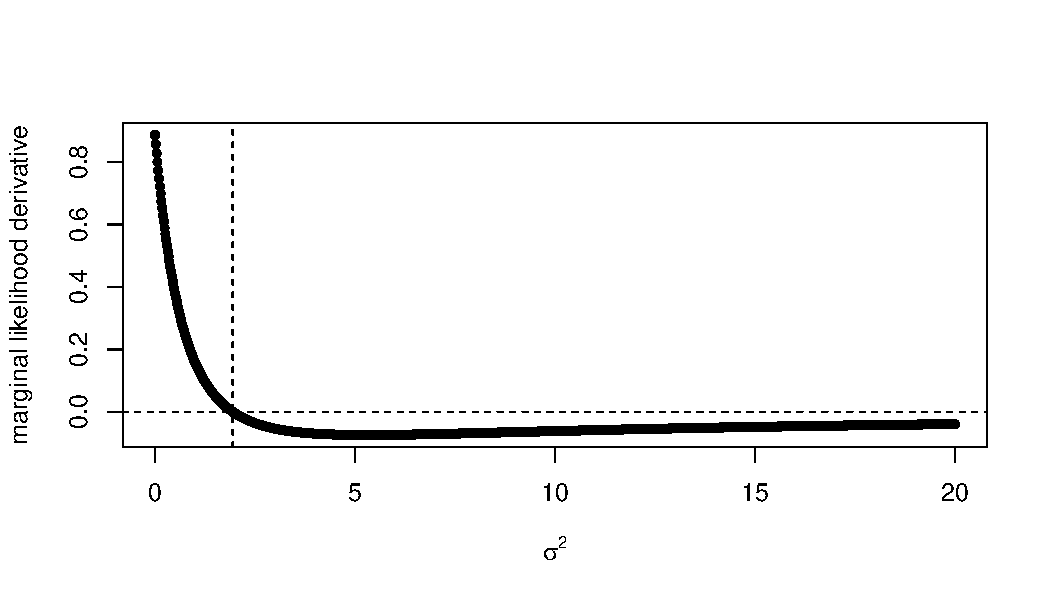
\includegraphics[width=\maxwidth]{figure/unnamed-chunk-3-1} 
\begin{kframe}\begin{alltt}
\hlcom{# function to draw samples from the predictive posterior}
\hlstd{draw_from_pred_posterior} \hlkwb{<-} \hlkwa{function}\hlstd{(}\hlkwc{number_samples}\hlstd{,} \hlkwc{y}\hlstd{,} \hlkwc{x}\hlstd{,} \hlkwc{xstar}\hlstd{,} \hlkwc{sigmaSq} \hlstd{=} \hlnum{1}\hlstd{)}
\hlstd{\{}

  \hlcom{# invert noisy K}
  \hlstd{K_y_inv} \hlkwb{<-} \hlkwd{solve}\hlstd{(}\hlkwd{kernel_fun}\hlstd{(x)} \hlopt{+} \hlkwd{diag}\hlstd{(}\hlkwd{rep}\hlstd{(sigmaSq,}\hlnum{2}\hlstd{)))}
  \hlcom{# get the other K's for new data}
  \hlstd{Kstar} \hlkwb{<-} \hlkwd{kernel_fun_pred}\hlstd{(x,xstar)}
  \hlstd{Kstarstar} \hlkwb{<-} \hlkwd{kernel_fun}\hlstd{(xstar)}
  \hlcom{# draw samples according to Ex. (d)}
  \hlkwd{rnorm}\hlstd{(number_samples,}
        \hlkwc{mean} \hlstd{=} \hlkwd{as.numeric}\hlstd{(}\hlkwd{t}\hlstd{(Kstar)} \hlopt \hlstd{K_y_inv} \hlopt \hlstd{y),}
        \hlkwc{sd} \hlstd{=} \hlkwd{sqrt}\hlstd{(}\hlkwd{as.numeric}\hlstd{(Kstarstar} \hlopt{-} \hlkwd{t}\hlstd{(Kstar)} \hlopt \hlstd{K_y_inv} \hlopt \hlstd{Kstar))}
  \hlstd{)}

\hlstd{\}}

\hlcom{# draw enough samples to get a feeling for the distribution}
\hlstd{samples_posterior} \hlkwb{<-}
       \hlkwd{draw_from_pred_posterior}\hlstd{(}\hlkwc{number_samples} \hlstd{=} \hlnum{1000}\hlstd{,} \hlkwc{sigmaSq} \hlstd{= bestSigmaSq}\hlopt{$}\hlstd{root,}
                                \hlkwc{y} \hlstd{= y,} \hlkwc{x} \hlstd{= x,} \hlkwc{xstar} \hlstd{=} \hlnum{0}\hlstd{)}
\hlcom{# plot the distribution}
\hlkwd{hist}\hlstd{(samples_posterior,} \hlkwc{breaks}\hlstd{=}\hlnum{50}\hlstd{,} \hlkwc{xlab}\hlstd{=}\hlkwd{expression}\hlstd{(y[}\hlstr{"*"}\hlstd{]}\hlopt{^}\hlstd{b))}
\end{alltt}
\end{kframe}
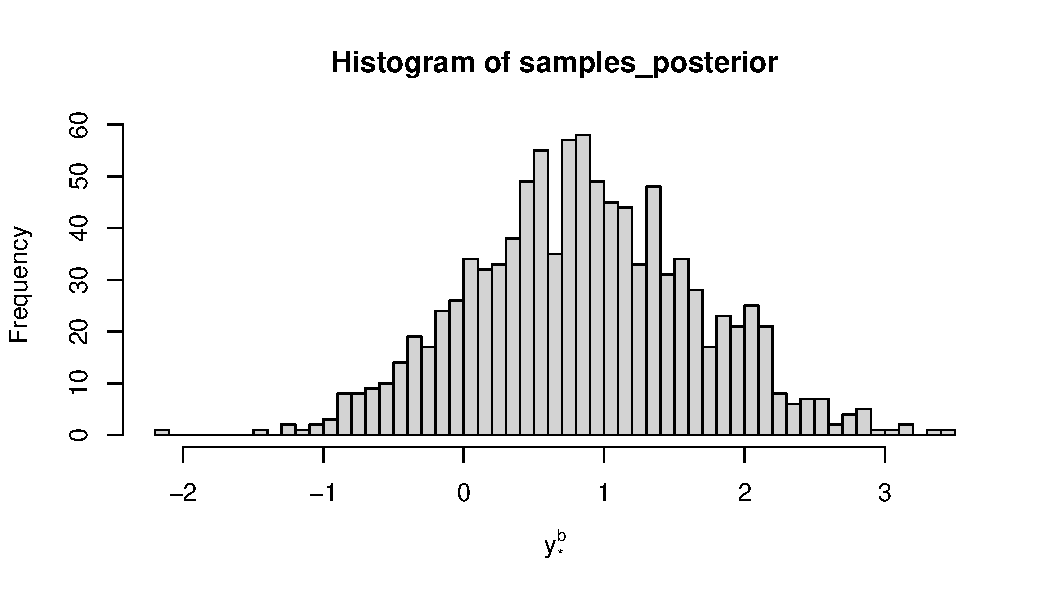
\includegraphics[width=\maxwidth]{figure/unnamed-chunk-3-2} 
\end{knitrout}

\end{enumerate}
}
\end{document}
